\documentclass[11pt]{amsart}
\usepackage{geometry}                % See geometry.pdf to learn the layout options. There are lots.
\geometry{letterpaper}                   % ... or a4paper or a5paper or ... 
%\geometry{landscape}                % Activate for for rotated page geometry
%\usepackage[parfill]{parskip}    % Activate to begin paragraphs with an empty line rather than an indent
\usepackage{graphicx}
\usepackage{amssymb}
\usepackage{amsmath}
\usepackage{epstopdf}
\usepackage{times, natbib, bm}
\DeclareGraphicsRule{.tif}{png}{.png}{`convert #1 `dirname #1`/`basename #1 .tif`.png}

\title{Relative performance of GAM and bootstrap uncertainty estimation in DSM}
\author{David L. Miller}
%\date{}                                           % Activate to display a given date or no date

\begin{document}
\maketitle


\section{Introduction}

This appendix gives a summary of a series of very simple simulations that were conducted to investigate the properties of the four methods of uncertainty estimation described in the article. These are:

\begin{itemize}
\item \textbf{Moving block bootstrap}: 
\item \textbf{Moving block bootstrap with detection function uncertainty}: 
\item \textbf{GAM uncertainty}:
\item \textbf{GAM uncertainty with variance propagation}:
\end{itemize}


\section{Scenarios}

Three (admittedly very simple) scenarios were tested; each consisted of a density based on a simple pattern. Creating a ``realistic'' scenario (e.g. including many covariates, correlation and so on) is not easy to construct and such a scenario would never encompass all of the possible combinations. As such, we decided to create three simple situations where it would be easy to discover whether there were difficulties with any of the above methods.

The underlying density surfaces are shown in Figure \ref{sim-plots}.

\begin{figure}[htbp]
\begin{center}
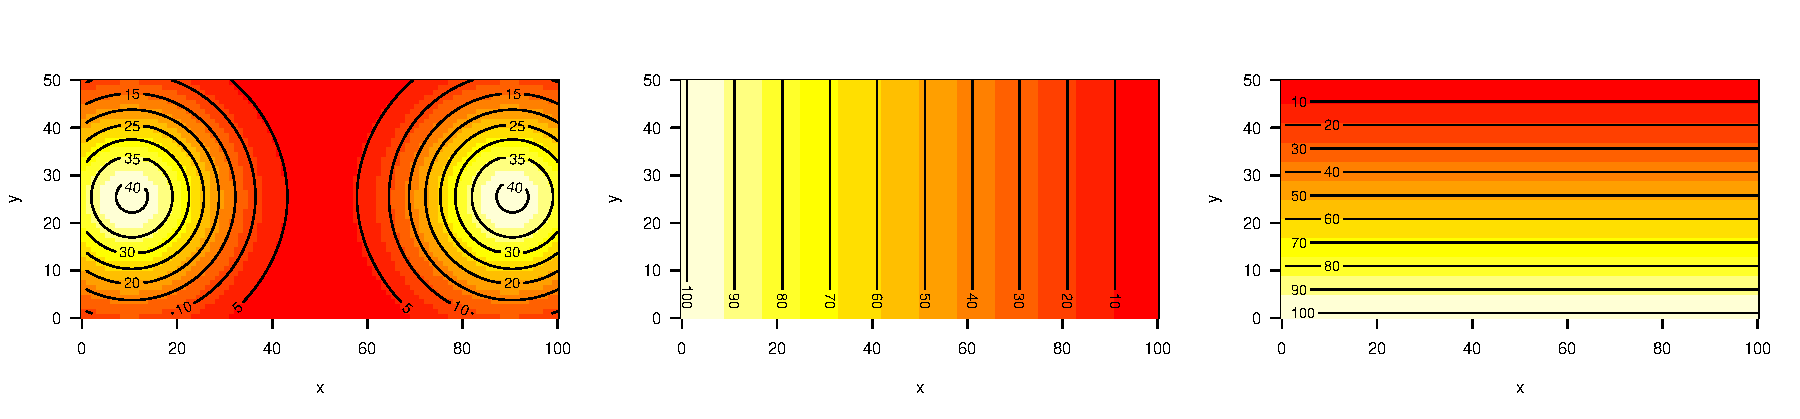
\includegraphics[width=\textwidth]{sim-plots.png}
\caption{The three underlying density surfaces used in the simulation.}
\label{sim-plots}
\end{center}
\end{figure}






\section{Results}


\section{Conclusion}




\bibliography{../dsm-refs.bib}


\end{document}  